\section{Methodology}

We will achieve the goal of estimating the dipole moment of several individual
grains per image in a semi-automatic fashion by dividing the task into three
parts that can be performed independently:

\begin{enumerate}
\item \textbf{Source detection and separation:} Identify and spatially isolate
  the magnetic field caused by each source. We will do this through a
  combination of classic potential field data processing (\textit{total
  gradient amplitude}) and image processing (histogram stretching and
  equalization) and segmentation methods (watershed segmentation).
\item \textbf{Position estimation}: Estimate the 3D position of a magnetic
  particle based on the magnetic field measurements and the assumption of a
  dipolar source. This can be achieved by applying the Euler Deconvolution
  method to the data segment identified in step 1.
\item \textbf{Magnetic moment inversion:} Estimate the 3-component dipole
  moment vector by inverting the magnetic field data using the position
  obtained from Euler Deconvolution as a constraint and the assumption of a
  dipolar source. This leads to a linear inverse problem that is stable and
  computationally efficient, particularly since the inversion is performed
  separately for each data segment identified in step 1.
\end{enumerate}

In the sections below, we describe the methodology used in each step of our
proposed workflow.

\subsection{Automatic source detection and separation}

Our first task is to automatically identify the signal of individual particles
and spatially segregate the data into windows, each containing the signal of a
single particle. We implemented the following workflow to achieve this:

\begin{enumerate}
\item Calculate the \textit{total gradient amplitude} (TGA), also known as the 3D analytic signal \citep{Roest1992Magnetic}, of the observed vertical   component of the magnetic field. The TGA is entirely positive and tends to be more concentrated on top of the magnetic field sources than the observed magnetic field. The derivative calculation also acts as a high-pass filter, removing long-wavelength noise from the data.
\item Apply a contrast stretching method to re-scale the TGA to a new range   defined by the lower and upper percentiles of the data in order to highlight the weaker signals, either coming from small or from deep-seated particles.
\item Use the Laplacian of Gaussian (LoG) method \citep{VanderWalt2014} on the   re-scaled TGA data to estimate the position and size of data windows containing the signal of each particle.
\end{enumerate}

The total gradient amplitude (TGA) was devised as a filter that can be applied
to aeromagnetic data to reduce the signal's dependence on the direction of
magnetization of the source and that concentrates the signal above the sources
\citep{Roest1992Magnetic, Nabighian2005}. The TGA is defined as the norm of the
gradient vector of a scalar field $f(x, y, z)$

\begin{equation}
\|\vec{\mathbf{\nabla}}f(x, y, z)\|  =
\sqrt{(\partial_x f)^2 + (\partial_y f)^2 + (\partial_z f)^2}
\ ,
\end{equation}

\noindent
in which $\partial_x f$ is the partial derivative of $f$ with respect to $x$
and likewise for the $y$ and $z$ directions. The partial derivatives are best
approximated using a second-order accurate central finite-difference scheme

\begin{equation}
\partial_x f(x, y, z) \approx
\dfrac{f(x + \Delta x, y, z) - f(x - \Delta x, y, z)}{2 \Delta x}
\ ,
\end{equation}

\noindent
and likewise for the $y$ and $z$ directions, in which $\Delta x$ is the grid
spacing (assumed to be equal in the $x$ and $y$ directions). For the $z$
component, $\Delta z = \Delta x$ and $f(x, y, z + \Delta z)$ and
$f(x, y, z - \Delta z)$ are calculated by upward and downward continuation,
respectively, performed in the wavenumber domain. The 2D maps of the $x$, $y$,
and $z$ derivatives will also be used in the Euler Deconvolution step described
below, which is known to be highly sensitive to noise in the derivatives
\citep{Saleh2012Applying}. This is why we prefer the finite-differences based
derivatives, which are less prone to amplifying short-wavelength noise than
those calculated in the wavenumber domain through the Fast Fourier Transform
(FFT).

Once we have obtained a TGA image, we apply a contrast stretching method to
re-scale the TGA values in order to highlight the weaker signals present in the
image. This is a necessary step to make sure that the blob detection algorithm
is able to identify particles causing both weak and strong signals. The
following contrast stretching operation is performed per pixel of the TGA image

\begin{equation}
\text{TGA}_{rescaled} =
2\left(\dfrac{\text{TGA} - v_{min}}{v_{max} - v_{min}}\right) - 1
\ ,
\end{equation}

\noindent
in which $v_{min}$ and $v_{max}$ are the upper and lower bounds of TGA values
that will be stretched to the range $[0, 1]$. By experimentation, we found
that values of $v_{min} = 1^\text{st}$ and $v_{max} = 99^\text{th}$
percentiles of the TGA range work well on real magnetic microscopy datasets.

The re-scaled TGA image is then used as input for a Laplacian of Gaussian (LoG)
blob detection algorithm \citep{Kong2013}. This method is able to identify the
location and size of multiple windows in the image containing ``blobs''. In our
case, the blobs are the re-scaled TGA field of each particle and the LoG method
detects the local TGA maxima. The LoG method is particularly well suited for
the detection of bright blobs on a dark background at the expense of a longer
computation time \citep{Han2016}. For the image sizes routinely found in
magnetic microscopy, the computation is fast and only needs to be performed
once per image.

\subsection{Euler Deconvolution}

Once the locations and sizes of the windows containing the isolated signals of
each particle are determined, we can apply the Euler Deconvolution (ED)
estimate of the $x$, $y$, and $z$ positions of the center of the particles
under a dipolar approximation. This technique was first proposed by
\citet{Thompson1982} under the name EULDPH and later extended to three
dimensions and renamed ``Euler Deconvolution'' by \citet{Reid1990}. ED is
traditionally performed on a set of moving windows that scan the entire
dataset, producing a large scatter of position estimates, most of which are
spurious \citep{Silva20033D}. This is only done because it is impractical to
segment an aeromagnetic dataset into individual anomalies. Fortunately,
magnetic microscopy images often contain fewer elongated features (e.g., dikes and
suture zones) and regional signals (e.g., Curie depth variations) that are
difficult to separate. This makes it possible for us to produce isolated
signals for each magnetic particle through the source detection step described
above. Since each data window contains only the signal of a single particle, we
are able to apply ED and generate only a single position estimate per particle.

\begin{figure}[tb]
\centering
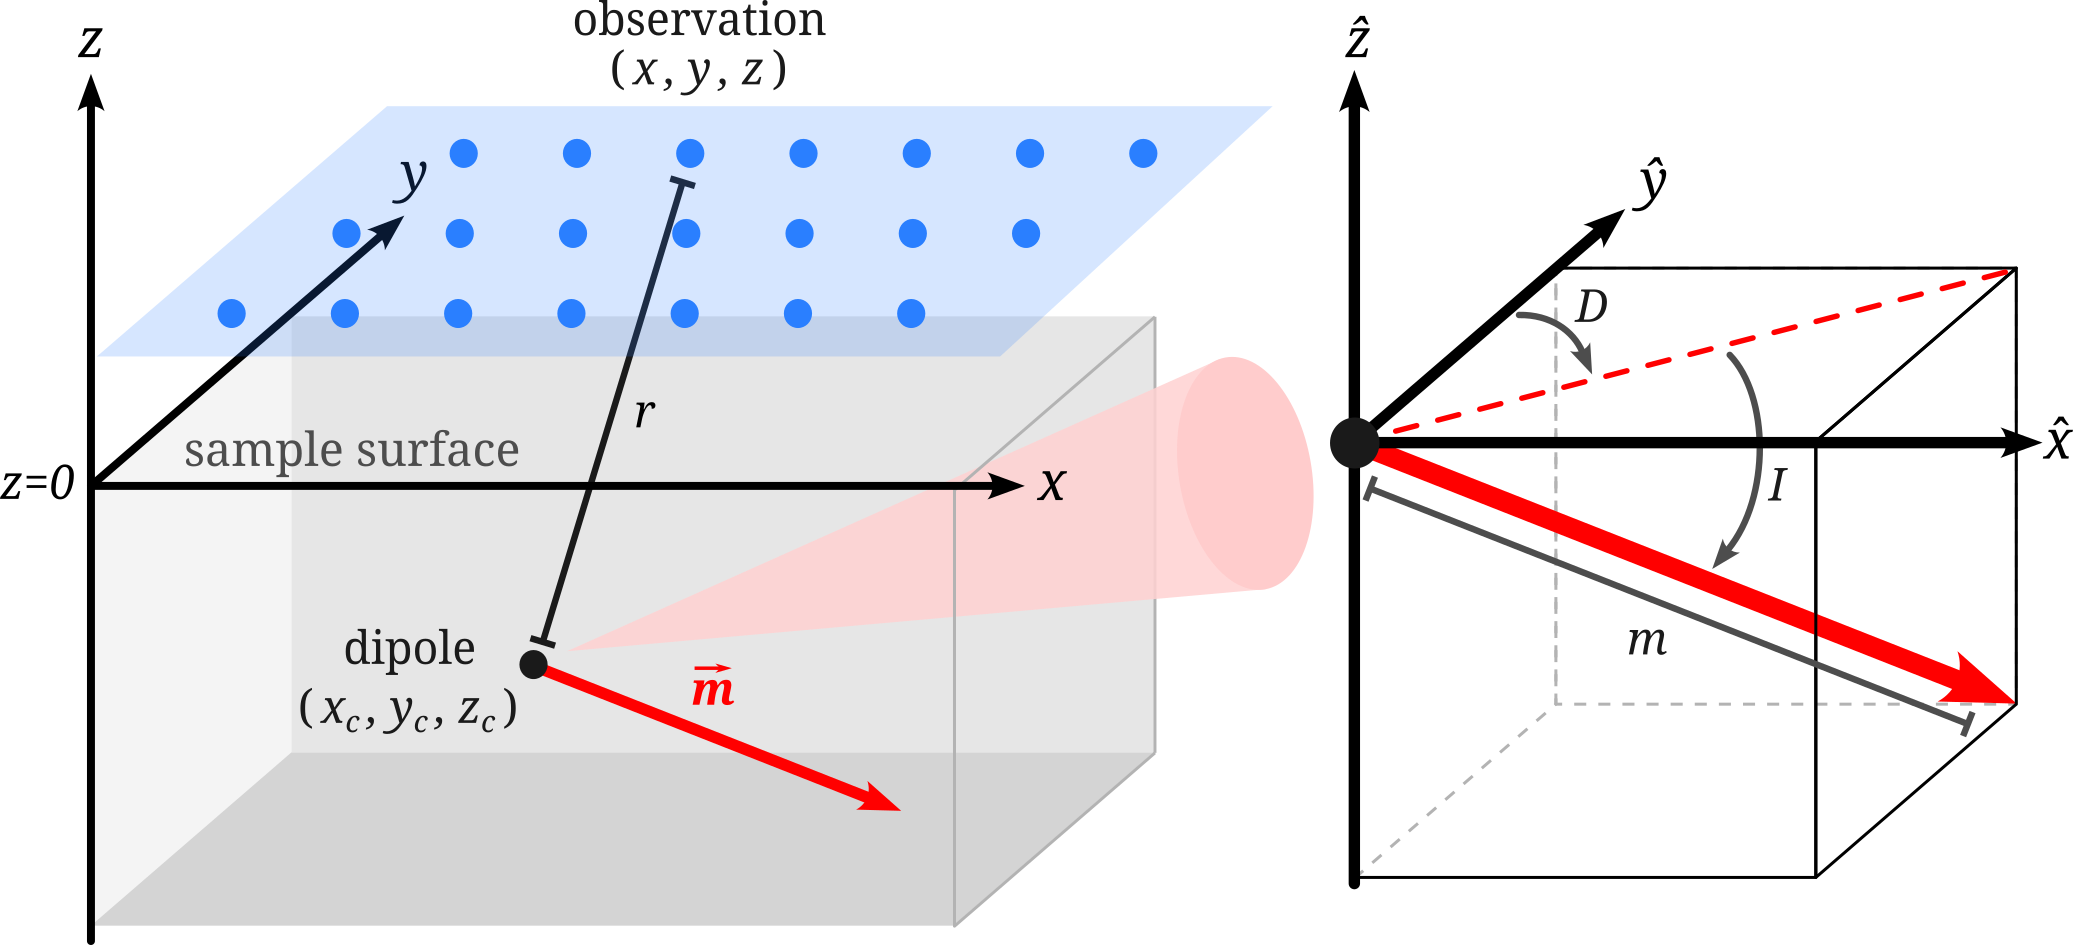
\includegraphics[width=\linewidth]{figures/coordinate-system-sketch.png}
\caption{
Schematic representation of the coordinates systems and modelling elements.
The left panel shows the $x, y, z$ right-handed coordinate system with $z$
pointing upward and away from the sample. The top surface of the sample defines
the $z=0$ surface. A dipole with dipole moment vector $\mathbf{\vec{m}}$ is
also shown at coordinates $(x_c, y_c, z_c)$. The observation points are located
at regular intervals on an $x-y$ plane at a positive $z$ separation from the
sample surface. The right panel zooms in on the dipole and shows the dipole
moment vector expressed in terms of inclination ($I$, positive downwards),
declination ($D$, angle with the $\hat{y}$ direction), and moment magnitude $m
= \|\mathbf{m}\|$.
}
\label{fig_coordinate_systems}
\end{figure}

Euler Deconvolution is formulated as a least-squares inversion of Euler's
homogeneity equation

\begin{equation}
\label{eq_euler_homogeneity}
(x - x_c)\partial_x f
+ (y - y_c)\partial_y f
+ (z - z_c)\partial_z f
= (b - f)\eta
\ ,
\end{equation}

\noindent
in which $(x_c, y_c, z_c)$ are the coordinates of the magnetic field source (Figure~\ref{fig_coordinate_systems}), $b$ is the base level representing a constant shift in the signal, and $\eta$ is the structural index corresponding to the nature of the source \citep{Reid1990}. This equation holds true for simple geometric sources, like spheres, dipoles, and vertical cylinders. Here, we assume that the magnetic particles are small enough and the sensor is far enough away that the sources can be represented by dipoles, yielding an $\eta=3$.

The inversion is performed by rearranging Equation~\ref{eq_euler_homogeneity} into a pseudo-parametric model with parameters $x_c$, $y_c$, $z_c$, and $b$

\begin{equation}
x_c \partial_x f + y_c \partial_x f + z_c \partial_x f + \eta b
=
x \partial_x f + y \partial_y f + z \partial_z f + \eta f
\ .
\end{equation}

Given a set of $N$ observations of the magnetic field as the harmonic function $f$ and its spatial derivatives, we can form the $N \times 4$ system of equations

\begin{equation}
\begin{bmatrix}
  {\partial_x f}_1 & {\partial_y f}_1 & {\partial_z f}_1 & \eta \\
  {\partial_x f}_2 & {\partial_y f}_2 & {\partial_z f}_2 & \eta \\
  \vdots & \vdots & \vdots & \vdots \\
  {\partial_x f}_N & {\partial_y f}_N & {\partial_z f}_N & \eta
\end{bmatrix}
\begin{bmatrix}
  x_c \\ y_c \\ z_c \\ b
\end{bmatrix}
=
\begin{bmatrix}
  x_1 {\partial_x f}_1 + y_1 {\partial_y f}_1 + z_1 {\partial_z f}_1 + \eta f_1 \\
  x_2 {\partial_x f}_2 + y_2 {\partial_y f}_2 + z_2 {\partial_z f}_2 + \eta f_2 \\
  \vdots \\
  x_N {\partial_x f}_N + y_N {\partial_y f}_N + z_N {\partial_z f}_N + \eta f_N \\
\end{bmatrix}
\ .
\end{equation}

In matrix notation, this linear system can be written as

\begin{equation}
\label{eq_euler_forward}
\mathbf{G} \mathbf{p} = \mathbf{h} \ .
\end{equation}

We can arrive at a solution to Equation~\ref{eq_euler_forward} by assuming that the three spatial derivatives of $f$ have negligible error and minimizing the misfit $\phi(\mathbf{p})$ between a pseudo-observation vector $\mathbf{h}^o$ and the predictions $\mathbf{h}$. The least-squares misfit $\phi(\mathbf{p})$ is defined as

\begin{equation}
\label{ZTSuSBbL16}
\phi(\mathbf{p}) = \|\mathbf{h}^o - \mathbf{h}\|^2 = (\mathbf{h}^o - \mathbf{G}\mathbf{p})^T (\mathbf{h}^o - \mathbf{G}\mathbf{p})\ .
\end{equation}

The minimum of $\phi(\mathbf{p})$ is obtained by solving the $4 \times 4$
system of normal equations

\begin{equation}
\mathbf{G}^T \mathbf{G} \mathbf{p} = \mathbf{G}^T \mathbf{h}^o\ .
\end{equation}

The solution vector $\hat{\mathbf{p}}$ provides an estimate of the position
$(x_c, y_c, z_c)$ and base level $b$ for the source located inside of a data
window. Repeating this process for each window produced by the source detection
algorithm will yield the horizontal locations and depths of each magnetic
particle.

\subsection{Magnetic moment inversion}

Once the source position is known and we can assume that it is approximately
spherical or dipolar, we can apply the method developed by
\citet{Oliveira2015Estimation} to estimate the dipole moment vector
$\mathbf{m}$ of the source. We begin by following
\citet{Oliveira2015Estimation} in formulating the magnetic induction vector
$\mathbf{b}$ of a dipole as

\begin{equation}
\label{eq_vector_dipole_field}
\mathbf{b}
=
\begin{bmatrix}
  b_x \\ b_y \\ b_z
\end{bmatrix}
= \dfrac{\mu_0}{4\pi}
\begin{bmatrix}
    \dfrac{\partial^2}{\partial x \partial x} \dfrac{1}{r}
  & \dfrac{\partial^2}{\partial x \partial y} \dfrac{1}{r}
  & \dfrac{\partial^2}{\partial x \partial z} \dfrac{1}{r}
  \\
    \dfrac{\partial^2}{\partial y \partial x} \dfrac{1}{r}
  & \dfrac{\partial^2}{\partial y \partial y} \dfrac{1}{r}
  & \dfrac{\partial^2}{\partial y \partial z} \dfrac{1}{r}
  \\
  \dfrac{\partial^2}{\partial z \partial x} \dfrac{1}{r}
  & \dfrac{\partial^2}{\partial z \partial y} \dfrac{1}{r}
  & \dfrac{\partial^2}{\partial z \partial z} \dfrac{1}{r}
\end{bmatrix}
\begin{bmatrix}
  m_x \\ m_y \\ m_z
\end{bmatrix}
= \dfrac{\mu_0}{4\pi} \mathbf{M}\,\mathbf{m}
\ ,
\end{equation}

\noindent
in which $r = \sqrt{(x - x_c)^2 + (y - y_c)^2 + (z - z_c)^2}$ is the Cartesian distance between the observation point $(x, y, z)$ and the source $(x_c, y_c, z_c)$ and $\mu_0$ is the vacuum magnetic permeability. Most magnetic microscopes provide measurements of only the vertical component $b_z$, which can be isolated from Equation~\ref{eq_vector_dipole_field} as shown in Equation~\ref{eq_dipole_bz}, which is a similar approach to the uniform model proposed by \cite{Weiss2007}.

\begin{equation}
\label{eq_dipole_bz}
b_z
= \dfrac{\mu_0}{4\pi}
\begin{bmatrix}
\dfrac{\partial^2}{\partial z \partial x} \dfrac{1}{r}
& \dfrac{\partial^2}{\partial z \partial y} \dfrac{1}{r}
& \dfrac{\partial^2}{\partial z \partial z} \dfrac{1}{r}
\end{bmatrix}
\begin{bmatrix}
m_x \\ m_y \\ m_z
\end{bmatrix}
= \dfrac{\mu_0}{4\pi} \mathbf{M_z}\,\mathbf{m}
\ .
\end{equation}

The three second-order derivatives in Equation~\ref{eq_dipole_bz} are

\begin{equation}
\begin{aligned}
\dfrac{\partial^2}{\partial z \partial x} \dfrac{1}{r} &=
\dfrac{3(z - z_c)(x - x_c)}{r^5}\ ,
\\
\dfrac{\partial^2}{\partial z \partial y} \dfrac{1}{r} &=
\dfrac{3(z - z_c)(y - y_c)}{r^5}\ ,
\\
\dfrac{\partial^2}{\partial z \partial z} \dfrac{1}{r} &=
\dfrac{3(z - z_c)^2}{r^5} - \dfrac{1}{r^3}\ .
\end{aligned}
\end{equation}

Given a set of $N$ observations of $b_z$ made inside a window containing a single source, we can form the $N \times 3$ linear equation system

\begin{equation}
\label{CgjOtKLQKT}
\begin{bmatrix}
\dfrac{\mu_0}{4\pi}\dfrac{3(z_1 - z_c)(x_1 - x_c)}{r_1^5}
& \dfrac{\mu_0}{4\pi}\dfrac{3(z_1 - z_c)(y_1 - y_c)}{r_1^5}
& \dfrac{\mu_0}{4\pi}\left(\dfrac{3(z_1 - z_c)^2}{r_1^5} - \dfrac{1}{r_1^3}\right)
\\
\dfrac{\mu_0}{4\pi}\dfrac{3(z_2 - z_c)(x_2 - x_c)}{r_2^5}
& \dfrac{\mu_0}{4\pi}\dfrac{3(z_2 - z_c)(y_2 - y_c)}{r_2^5}
& \dfrac{\mu_0}{4\pi}\left(\dfrac{3(z_2 - z_c)^2}{r_2^5} - \dfrac{1}{r_2^3}\right)
\\
\vdots & \vdots & \vdots
\\
\dfrac{\mu_0}{4\pi}\dfrac{3(z_N - z_c)(x_N - x_c)}{r_N^5}
& \dfrac{\mu_0}{4\pi}\dfrac{3(z_N - z_c)(y_N - y_c)}{r_N^5}
& \dfrac{\mu_0}{4\pi}\left(\dfrac{3(z_N - z_c)^2}{r_N^5} - \dfrac{1}{r_N^3}\right)
\end{bmatrix}
\begin{bmatrix}
m_x \\ m_y \\ m_z
\end{bmatrix}
=
\begin{bmatrix}
{b_z}_1 \\ {b_z}_2 \\ \vdots \\ {b_z}_N
\end{bmatrix}
\ ,
\end{equation}

\noindent
which can also be expressed in matrix form as

\begin{equation}
\label{qdhqM4s9Ln}
\mathbf{A} \mathbf{m} = \mathbf{d} \ .
\end{equation}

As with Euler Deconvolution, we can find a dipole moment vector that best fits
a set of $N$ observations of the vertical component of the magnetic field
$\mathbf{d}^o$ in a least-squares sense by minimizing the misfit function

\begin{equation}
\label{uV9pRVYO4l}
\Gamma (\mathbf{m}) = \| \mathbf{d}^o - \mathbf{d} \|^2 = (\mathbf{d}^o - \mathbf{A}\mathbf{m})^T  (\mathbf{d}^o - \mathbf{A}\mathbf{m})\ .
\end{equation}

\noindent
The dipole moment vector that minimizes $\Gamma (\mathbf{m})$ can be found by
solving the $3 \times 3$ normal equation system

\begin{equation}
\mathbf{A}^T \mathbf{A} \mathbf{m} = \mathbf{A}^T\mathbf{d}^o\ .
\end{equation}

\noindent
The estimated dipole moment vector $\hat{\mathbf{m}}$ can be converted into declination $D$, inclination $I$, and magnitude $m$, which are more intuitive quantities for interpreting paleomagnetic results, like so \citep{Tauxe2018}

\begin{equation}
\label{eq_vector_to_incdec}
\begin{aligned}
I &= \tan^{-1}\dfrac{m_z}{\sqrt{m_x^2 + m_y^2}} \ , \\
D &= \tan^{-1}\dfrac{m_x}{m_y} \ , \\
m &= \sqrt{m_x^2 + m_y^2 + m_z^2} \ .
\end{aligned}
\end{equation}

\noindent
It is important to note that these are not paleomagnetic declination and inclination angles, but are instead related to the sample coordinate system. To obtain the paleomagnetic direction, the dipole moment vector must be rotated to the sample field orientation prior to the application of Equation~\ref{eq_vector_to_incdec}.

In a micromagnetic survey, or any geophysical survey, measurements are affected by noise caused by experimental errors, equipment inaccuracies, and sensor limitations. This noise will affect the estimated parameter vector $\mathbf{\hat{m}}$, regardless of the method used. Assuming that the noise in the observed data is independent and normally distributed with zero mean and variance ${\sigma_0}^2$, we can estimate the variance of the parameters by propagation of uncertainties. In reality, the data variance  ${\sigma_0}^2$ is rarely known and must be estimated using the $\chi^2$ statistic \citep{Aster2019}

\begin{equation}
\label{eq_chi_square}
\hat{\sigma}_0^2 = {\chi}^2 = \dfrac{\|\mathbf{d}^o - \mathbf{A}\hat{\mathbf{m}}\|^2}{N - 3}\ ,
\end{equation}

\noindent
in which $N - 3$  are the degrees-of-freedom.
The covariance matrix $\mathbf{C}$ of the estimated parameters is then given by \citep{Aster2019}

\begin{equation}
\label{eq_covariance}
\mathbf{C}
=
\hat{\sigma}_0^2 (\mathbf{A}^T\mathbf{A})^{-1}
=
\begin{bmatrix}
\sigma_x^2 & \sigma_{xy} & \sigma_{xz} \\
\sigma_{yx} & \sigma_y^2 & \sigma_{yz} \\
\sigma_{zx} & \sigma_{zy} & \sigma_z^2
\end{bmatrix}
\ .
\end{equation}

\noindent
From the main diagonal of $\mathbf{C}$, we can obtain the variances of the
estimated declination $\sigma_D^2$, inclination $\sigma_I^2$, and magnitude $\sigma_m^2$
by propagation of uncertainties from Equation~\ref{eq_vector_to_incdec}

\begin{equation}
\label{eq_variances}
\begin{aligned}
\sigma_D^2 &= \dfrac{m_y^2\sigma_x^2 + m_x^2\sigma_y^2}{\left(m_x^2 + m_y^2\right)^2} \ , \\
\sigma_I^2 &= \dfrac{m_x^2 m_z^2 \sigma_x^2 + m_y^2 m_z^2 \sigma_y^2 + \left(m_x^2 + m_y^2\right)^2\sigma_z^2}{\left(m_x^2 + m_y^2\right) m^4} \ , \\
\sigma_m^2 &= \dfrac{m_x^2\sigma_x^2 + m_y^2\sigma_y^2 + m_z^2\sigma_z^2}{m^2} \ .
\end{aligned}
\end{equation}

\noindent
These variances reflect the sensitivity of the estimated dipole moment to random noise in the magnetic field observations. However, they do not capture other, often larger, sources of uncertainty like systematic errors in the observations, data positioning errors, and the validity of the dipolar approximation. Therefore, we recommend that these estimated variances be treated with caution and should not be interpreted as ``the degree of certainty that the estimated values are the true values''.

Parameters retrieved during inversion procedures may not always explain the observed data perfectly.
Hence, it is necessary to evaluate how well the predicted data is able to fit the observed data.
When evaluating the goodness of fit of inversions of magnetic microscopy data, \citet{Fu2020} apply a ``dipolarity parameter'' ($D$).
We note that $D$ is equivalent to the coefficient of determination

\begin{equation}
\label{eq_r2}
R^2 = 1 - \dfrac{\|\mathbf{d}^o - \mathbf{A}\hat{\mathbf{m}}\|^2}{\|\mathbf{d}^o - \bar{b}_z^o\|^2}\ ,
\end{equation}

\noindent
in which $\bar{b}_z^o$ is the mean of the observed data.
$R^2$ has a maximum value of 1, which indicates a perfect fit of the data.
Values close to 1 can therefore be interpreted to mean that a simple dipole model is able to explain the observed data.
On the other hand, low values of $R^2$ indicate that the dipole model is not able to explain the observed data.

\citet{CortesOrtuno2021} use the ``signal-to-noise ratio'' (SNR) to evaluate the goodness of fit.
Here, we define the SNR in a logarithmic decibel scale to make it independent of the scale of the data

\begin{equation}
\label{eq_snr}
\text{SNR} = 10 \log_{10}\dfrac{\sigma^2_d}{\sigma^2_r}\ ,
\end{equation}

\noindent
in which $\sigma^2_d$ is the variance of the observed data and $\sigma^2_r$ is the variance of the residuals $\mathbf{r} = \mathbf{d}^o - \mathbf{A}\hat{\mathbf{m}}$.
The SNR is the trade-off between the signal and its associated noise, which we approximate by the inversion residuals.
The higher the SNR values (in decibels), the better the fit to the observed data.
For a signal to be ``visible'', \citet{Strum2014} suggest that $\text{SNR} \ge 3$, which means the signal is at least three times stronger than the noise.
Here, we use both $R^2$ and SNR as criteria for filtering out unreliable estimates from our dipole moment inversions.